\begin{figure}[H]
  \centering
  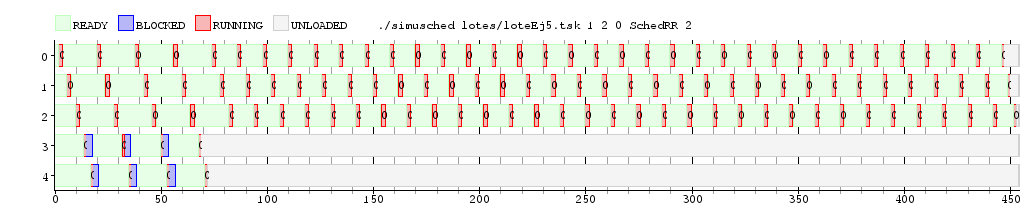
\includegraphics[width=1\textwidth]{img/imgEj5-1}
  \caption{}
  \label{fig:ej5-1}
\end{figure}

\begin{figure}[H]
  \centering
  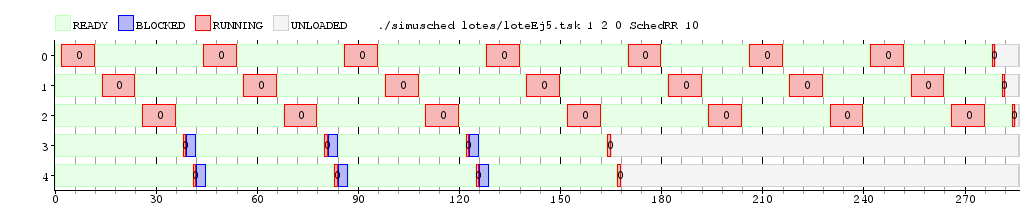
\includegraphics[width=1\textwidth]{img/imgEj5-2}
  \caption{}
  \label{fig:ej5-2}
\end{figure}

\begin{figure}[H]
  \centering
  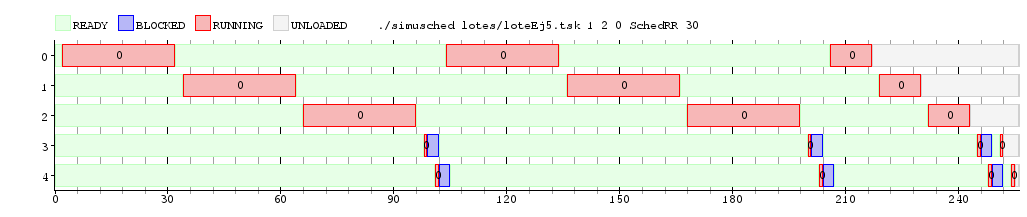
\includegraphics[width=1\textwidth]{img/imgEj5-3}
  \caption{}
  \label{fig:ej5-3}
\end{figure}

\begin{table}[H]
  \center
  \begin{center}
  \begin{tabular}{c|c|c|c|}
    \cline{2-4}
    & \multicolumn{3}{|c|}{\cellcolor{LightCyan}Latencia} \\
    \hline
    \rowcolor{LightCyan}
    \multicolumn{1}{|c|}{Quantum} & 2 & 10 & 30 \\
    \hline
    \multicolumn{1}{|c|}{\cellcolor{LightCyan}Tarea 0} & 2 & 2 & 2 \\
    \multicolumn{1}{|c|}{\cellcolor{LightCyan}Tarea 1} & 6 & 14 & 34 \\
    \multicolumn{1}{|c|}{\cellcolor{LightCyan}Tarea 2} & 10 & 26 & 66 \\
    \multicolumn{1}{|c|}{\cellcolor{LightCyan}Tarea 3} & 15 & 39 & 99 \\
    \multicolumn{1}{|c|}{\cellcolor{LightCyan}Tarea 4} & 18 & 42 & 101 \\
    \hline
    \multicolumn{1}{|c|}{\cellcolor{LightCyan}Promedio} & 10.2 & 24.6 & 60.4 \\
    \hline
  \end{tabular}
  \end{center}
  \caption{\footnotesize Latencia de cada tarea y latencia promedio según la duración del \emph{quantum} utilizado.}
  \label{tab:ej5-1}
\end{table}

\begin{table}[H]
  \center
  \begin{center}
  \begin{tabular}{c|c|c|c|}
    \cline{2-4}
    & \multicolumn{3}{|c|}{\cellcolor{LightCyan}\emph{Waiting time}} \\
    \hline
    \rowcolor{LightCyan}
    \multicolumn{1}{|c|}{Quantum} & 2 & 10 & 30 \\
    \hline
    \multicolumn{1}{|c|}{\cellcolor{LightCyan}Tarea 0} & ? & ? & ? \\
    \multicolumn{1}{|c|}{\cellcolor{LightCyan}Tarea 1} & ? & ? & ? \\
    \multicolumn{1}{|c|}{\cellcolor{LightCyan}Tarea 2} & ? & ? & ? \\
    \multicolumn{1}{|c|}{\cellcolor{LightCyan}Tarea 3} & ? & ? & ? \\
    \multicolumn{1}{|c|}{\cellcolor{LightCyan}Tarea 4} & ? & ? & ? \\
    \hline
    \multicolumn{1}{|c|}{\cellcolor{LightCyan}Promedio} & ? & ? & ? \\
    \hline
  \end{tabular}
  \end{center}
  \caption{\footnotesize Tiempo total de ejecución de cada tarea (\emph{turn-around}) y promedio según la duración del \emph{quantum} utilizado.}
  \label{tab:ej5-2}
\end{table}

\begin{table}[H]
  \center
  \begin{center}
  \begin{tabular}{c|c|c|c|}
    \cline{2-4}
    & \multicolumn{3}{|c|}{\cellcolor{LightCyan}\emph{Turn-around}} \\
    \hline
    \rowcolor{LightCyan}
    \multicolumn{1}{|c|}{Quantum} & 2 & 10 & 30 \\
    \hline
    \multicolumn{1}{|c|}{\cellcolor{LightCyan}Tarea 0} & 447 & 279 & 217 \\
    \multicolumn{1}{|c|}{\cellcolor{LightCyan}Tarea 1} & 450 & 282 & 230 \\
    \multicolumn{1}{|c|}{\cellcolor{LightCyan}Tarea 2} & 453 & 285 & 243 \\
    \multicolumn{1}{|c|}{\cellcolor{LightCyan}Tarea 3} & 69 & 165 & 252 \\
    \multicolumn{1}{|c|}{\cellcolor{LightCyan}Tarea 4} & 72 & 168 & 255 \\
    \hline
    \multicolumn{1}{|c|}{\cellcolor{LightCyan}Promedio} & 298.2 & 235.8 & 239.4 \\
    \hline
  \end{tabular}
  \end{center}
  \caption{\footnotesize Tiempo total de ejecución de cada tarea (\emph{turn-around}) y promedio según la duración del \emph{quantum} utilizado.}
  \label{tab:ej5-3}
\end{table}

%EN el primer caso gasto lo mismo en CS que en CPU